\documentclass[runningheads]{llncs}
%
\usepackage[T1]{fontenc}
% T1 fonts will be used to generate the final print and online PDFs,
% so please use T1 fonts in your manuscript whenever possible.
% Other font encondings may result in incorrect characters.
%
\usepackage{graphicx}
% Used for displaying a sample figure. If possible, figure files should
% be included in EPS format.
%
% If you use the hyperref package, please uncomment the following two lines
% to display URLs in blue roman font according to Springer's eBook style:
%\usepackage{color}
%\renewcommand\UrlFont{\color{blue}\rmfamily}
%
\begin{document}
%
\title{A domain-driven distributed reference architecture for big data systems}
%
%\titlerunning{Abbreviated paper title}
% If the paper title is too long for the running head, you can set
% an abbreviated paper title here
%
% \author{Pouya Ataei\inst{1,2,3}\orcidID{0000-0002-0993-3574} \and
% Alan Litchfield\inst{1,4,5}\orcidID{0000-0002-3876-0940}}
%
% \authorrunning{F. Author et al.}
% First names are abbreviated in the running head.
% If there are more than two authors, 'et al.' is used.
%
% \institute{Auckland University of Technology, Auckland, New Zealand \and
% \email{pouya.ataei@aut.ac.nz}\and
% School of Engineering, Computer and Mathematical Sciences\and
% \email{alan.litchfield@aut.ac.nz} \and
% Service and Cloud Computing Research Lab}
%
\maketitle              % typeset the header of the contribution
%
\begin{abstract}
    The proliferation of digital devices, rapid development of softwares and the infrastructure of today, have augmented user’s capability to produce at an unpredecented
    rate. This has precipitated a shift in the industry and dawned a new era, the era of
    big data. The era of big data began when the variety, velocity and volume of data
    overwhelmed traditional systems, and induced a paradigm shift in data engineering.
    Whereas many companies attempted to harness the benefits of big data, success rates
    are scarce. According to several sources, it has been estimated that only 20\% of companies have successfully institutionalised big data. This is due to several challenges such
    as rapid technology change, organisational culture, complexities of data engineering,
    system development and big data architecture. The aim of this study is to facilitate
    the areas of big data architecture, data engineering and system development by introducing a domain driven distributed big data reference architecture. This artefact is
    developed following the guidelines for an empirically grounded reference architecture
    and has been evaluated in a real-world scenario. A prototype of the artefact has been
    instantiated and applied to solve a problem in practice. The results display a good degree of utility and applicability, alongside thought-proving architectural tradeoffs and
    challenges.

\keywords{Big data architecture  \and Big data reference architecture \and Big data \and Data engineering \and Distributed systems.}
\end{abstract}
%
%
%
\section{Introduction}
The ubiquity of digital devices and proliferation of software applications have augmented users to generate data at an unprecedented rate. In this day and age, almost all aspects of human life is integrated with some sort of software system, that by large, is processing data, and executing the necessary computations. 

According to Internetlivestats.com \cite{internet2019internet} in one second 3,135,050 emails are sent, 1,151 Instagram photos are uploaded, 6,738 Skype calls are made and 147,084 GB of traffic has gone through the internet. That is, in the last minute, 825.04 terabytes have been transferred through the internet.The rapid expansion and evolution of data from a structured element that is passively stored in the database to something that is used to support proactive decision making for business competitive advantage, have dawned a new era, the era of Big Data (BD). The era of BD began when velocity, variety and volume of data overwhelmed traditional systems used to process that data \cite{ataei2021neomycelia}\cite{AtaeiACIS}. 

BD is the practice of crunching large sets of heterogenous data to discover patterns and insights for business competitive advantage \cite{AtaeiHype}. Since the inception of the term, ideas have ebbed and flowed along with the rapid advancements of technology, and many strived to harness the power of data. Nevertheless, BD is not a magical wand that can enchant any business processes and many have failed to absorb the complexity of this new field. According to a recent survey by MIT Technology Review insights in partnership with Databricks, only 13\% of organizations excel at delivering on their data strategy. Another survey by NewVantage Partners highlighted that only 24\% of organizations have successfully adopted BD \cite{NewVantageSurvey}. 

Sigma computing report indicated that 1 in 4 business experts have given up on getting insights they needed because the data analysis took too long \cite{SigmaSurvey}. Along the lines, McKinsey \& Company \cite{analytics2016age} and Gartner \cite{GartnerSury} demonstrated that approximately only 20\% of organizations have fully adopted BD. These statistics unveil the truth that successful adoption of BD system is scarce. Among the challenges of adopting BD, the most highlighted are "cultural challenges of becoming data-driven", "BD architecture", "data engineering complexities", "rapid technology change", and "lack of sufficiently skilled data engineers" \cite{AtaeiBigDataEnvirons}. 

% In the past, organizations relied on a few technology giants to account for their analytics and storage needs, whereas today's ecosystem of BD encompasses far-reaching plethora of technologies ranging from visualization to high-level sql-like scripting languages to logging, stream processing and distributed storage. 

% On the other hand, in react years, more and more companies are shifting to cloud native architectures for improved efficiency, cost reduction, which in turn led to creation of new roles such as chief data officers (CDOs) and chief analytic analytics officer (CAOs) to channel the organizational BD capabilities towards fruition and competitive advantage. 

% Taking all into consideration, how can one embark on such rather sophisticated journey? what is best initial point for adopting BD ? what can be a good logical approach to address the ever-increasing complexity of BD systems? how can the organization develop a BD system that can effectively handle data of various workloads such as business analytics, real-time stream processing, bulk batch processing and machine learning ? 

A big data system is motivated by an array of functional requirements and quality goals. But if this system is to be successful, it must achieve these functional requirements within an acceptable performance, availability, modifiability and cost parameters. The software architecture is the key ingredient in determining whether these goals are attainable, before colossal amount of resources are committed to it. The initial design, development and deployment of a BD system does not mean success. As system grows larger, data providers and data consumers increase, data variety expands, data velocity extends, and metadata become increasingly more challenging to handle. This means, only a handful of hyper-specialized data engineers would be able to understand the system internal, resulting in silos, burnt out and potential miscommunication. 

This creates a perfect ground for immature architectural decisions that result in hard-to-main and hard-to-scale systems, and raise high-entry blockage. Since ad-hoc BD designs are undesirable and leaves many engineers and architects in the dark, novel architectures that are specifically tailored for BD are required. To contribute to this goal, we explore the notion of reference architectures (RAs) and presented a domain-driven distributed software RA for BD systems.

\section{Why Reference Architecture?}
% To rationalize why we have chosen RAs as the suitable artefact, we first have to clarify two underlying assumptions: 1) a sound software architecture is integral to successful development and maintenance of software systems, and 2) there is a substantial body of knowledge in the field of software architecture to support the development of an effective RA.

In essence, software architecture is an artefact that aims to satisfy business objectives through a software solution that is evolvable, const-efficient, maintainable, and scalable. In addition, it allows for capturing design issues when they are still cheap. Whereas this practice can be applied to any class of systems, it's particularly highlighted when it comes to design and development of complex system such as BD \cite{ataei2021neomycelia}. Despite the known complexity of BD systems, good news is that a RA can be developed, analyzed and designed to incorporate best practices, techniques and patterns that will support the achievement of BD undertakings. This can help engineers and architect better absorb complexity of BD system development and make it tractable. 

This approach to system development is not new to practitioners of complex system. In software product line (SPL) development, RAs are utilized as generic artifacts that are instantiated and configured for a particular domain of systems \cite{Derras}. In software engineering, IT giants like IBM have referred to RAs as the 'best of best practices' to address complex and unique system design challenges \cite{Cloutier}. In other international standardization, RAs have been repeatedly used to standardize an emerging domain, a good example of this is BS ISO/IEC 18384-1 RA for service oriented architectures \cite{Iso18384-1}. RAs are used for political speech and even NASA space data systems \cite{NASA}.

Based on the premises discussed above, RAs can be considered effective for addressing the complexity of BD system development for the following reasons; 1) RAs promote adherence to best practices, patterns, and standards, 2) RAs can endow the architecture team with increased openness and interoperability, incorporating architectural patterns that ensue desirable predefined quality attributes, 3) RAs can serve as the locus of communication, bringing various stakeholders together. 

% 4) RAs can be effective in identification and addressing of cross-cutting concerns, 5) RAs can be some of the best approaches to complex system development such as BD, capturing design problems when they are still cheap, 6) RAs can take the role of blueprint and summary in the portfolio of software architects and data engineers, resulting in better dissemination of knowledge, 7) RAs can manifest the implicit knowledge of software architects as explicit actionable models.

\section{Research Methodology}
There are several approaches to systematic development of RAs. In one effort, Cloutier et al \cite{Cloutier} demonstrated a high-level model for development of RAs through collection of contemporary architectural patterns and advancements. In another effort, Bayer et al \cite{bayer1999pulse} introduced a method for creation of RAs for product line development called PuLSE DSSA. Stricker et al \cite{stricker2010creating} presented the idea of pattern based RA for service based systems and used patterns as first class citizens. Along the lines, Nakagaw et al \cite{nakagawa2014consolidating} presented a four-step approach to design and development of RAs. In a more recent study, Derras et al \cite{Derras} presented a four-phase approach for practical RA development in the context of domain engineering and software product line. This approach is influenced by ISO/IEC 26550 \cite{wg2015iso}.

% Clouterier's approach is driven from the Stevens Institute of Technology forum for systems engineers and tend to explicate RAs from a system engineering point of view. 



% This methodology is inspired by the works of Kazman et al \cite{kazman1994saam} and in specific their architecture evaluation method; SAAM. 

% Therefore it tends to pivot around scenarios for creation of candidate architectures which results in the intended RA. 



% This study, inspired by the works of Buschmann \cite{buschmann1996pattern}, and Gamma et al \cite{gamma1995design} portrays the RA as amalgamation of various patterns that are structured into different categories namely; high-level patterns, abstract patterns, and implementation patterns. This study is part of the NEXOF-RA \cite{birukounexof} project. 



% This methodology benefits from an ecosystem of complementary artifacts that facilitate the process of RA development, such as the RAModel \cite{nakagawa2012ramodel} (a reference model), and FERA \cite{santos2013checklist} (a checklist for evaluation of RAs). 



Nguyen et al utilized reverse engineering and reference model for creation of agent systems reference architecture \cite{nguyen2010methodology}, and Norta \cite{norta2006developing} followed a pattern based approach similar to that of Stricket et al. Galster and Avgeriou \cite{GALSTER} proposed a 6 step methodology that is founded on two major concepts; 1) empirical foundation and 2) empirical validity.

Analysis and study of these methodologies for design and development of RAs have highlighted several recurring themes.
%  While some of the these studies are older and some are more recent, observed commonalities are similar.
All these methodologies share the same fundamental pillars that 1) RAs should capture the essence of best practices, 2) RAs can be built by absorbing current best practices, standards, architectures, RAs, and systems, 3) RAs should sit at the right level of abstraction,
%  and 4) RAs should be communicated effectively. 

Taking all these into consideration, we found 'Empirically-grounded reference architectures' methodology proposed by Galster and Avgeriou as the suitable methodology for the purposes of this study. This decision is due to two factors; 1) this methodology is the most adopted approach for RA development, and 2) the focal elements surrounding the methodology is in-line with the objectives of this study. 

Nevertheless, this methodology suffered from a few limitations and we had to augment several areas of it with other approaches in order to arrive at the desired rigour and relevance. For instance, we could not find comprehensive guidelines on how to collect empirical data in step 3 of the methodology. We did not know what kind of theory we should collect and how should we model the data collected. Lack of systematicity and transparency on this area, would undermine our overall approach, therefore we employed Nakagawa et al's information source investigation guidelines and the idea of RAModel \cite{nakagawa2012ramodel}. 

Another area were we faced limitation was evaluation. The methodology did not provide detailed instructions on evaluation of the RA, thus, we looked for a more systematic and stronger evaluation approach. For this purposes, we first instantiated a prototype of the RA in a real world practice and then used the 'Architecture Tradeoff Analysis Method (ATAM)'\cite{KazmanATAM} to evaluate the artefact.

The methodology chosen for this study is constituent of 6 steps which are respectively; 1) Decision on type of the RA, 2) Design strategy, 3) Empirical acquisition of data, 4) Construction of the RA, 5) Enable RA with variability, 6) Evaluation of the RA. 

% It is essential to clarify that the phrase 'empirically grounded' refers to two concepts; 1) RA should be based on well-established and proven principles, and 2) RAs should be evaluated for validity and applicability. These concepts do not only belong to the works of Galster and Avgeriou; other researchers such as Derras et al \cite{Derras} and Cloutier et al \cite{Cloutier} have promoted the same ideologies. 

% Lastly, it is worth mentioning that this research methodology is iterative, implying that the results yielded from the last step (evaluation) will determine the subsequent iteration until the artefact reaches saturation (research objectives).

\subsection{Step 1: Decision on type of the RA}
Precursor to development of the RA, it's effective to determine the type of it. The type is an important factor as it illuminates on the structure, the data to be collected and objective of the RA. To determine the type of the RA, we used the classification framework provided by Angelov et al \cite{angelov2009classification} and the SLR conducted by Ataei et al \cite{AtaeiACIS}. 

% This classification is made up of five major RA types based on three major dimensions namely goal, context, and design. These dimensions each have their own sub-dimensions. Dimensions and sub-dimensions are derived by the means of interrogatives.

In this classification framework, RAs are categorized in two major groups; 1) standardization RAs, and 2) facilitation RAs. The study provides a good list of available RAs for different categories, which helps with clarification. 

The domain driven distributed RA chosen for the purposes of this study pursues two essential goals; 1) openness and interoperability between different heterogenous components of BD ecosystem and 2) facilitation of BD system development and data engineering. Accordingly, the output artefact is classified as 'classical standardization RA designed to be implemented in multiple organizations'. 

\subsection{Step 2: Selection of Design Strategy}
According to Galster et al \cite{GALSTER}, RAs can have two major design strategies to them; 1) RAs that are based on existing patterns, principles and architectures, and 2) RAs that are developed from scratch. Designing RAs from scratch is scarce and usually happens in areas that have received no attention (could be BD in 2004). On the other hand, RAs are proven more successful when built from the proven practices \cite{Cloutier}. 

The RA developed for the purposes of this study is a research-based RA based on existing RAs, concrete architectures, patterns, standards and best practices.

\subsection{Step 3: Empirical Acquisition of Data}
Due to limitations witnessed by the Galster et al's methodology, we have augmented this phase to increase transparency and systematicity, by employing a systematic literature review (SLR) for data collection. 

This phase is comprising of three major undertakings; 1) identification of data sources, 2) capturing data from the selected sources and 3) synthesis of the selected data. 

\subsubsection{Identification of Data Sources\\}

For this sub-phase, we employed the ProSA-RA's 'information sources investigation'. 

% This has provided us with guidelines necessary to capture ancillary and focal knowledge and theories necessary to understand the target domain, which laid the foundation of the RA development. 

To unearth the essential architectural quanta, we selected our sources as 'publications'. In order to capture the essence of existing body of knowledge from publications, we conducted a systematic literature review (SLR) following the guidelines of PRISMA presented by Moher et al \cite{Shamseer}. The main objective of this SLR is to find common architectural constructs among existing BD architectures. This SLR is an extension of Ataei et al work \cite{AtaeiACIS} which covered all the RAs by 2020. 

We followed the exact methodology as described in \cite{AtaeiACIS}, but this time for the years 2021 and 2022. 

% Databases chosen for this SRL includes ScienceDirect, IEEE Explore, SpringerLink, ACM
% library, MIS Quarterly, Elsevier, AISel as well as citation databases such as Scopus, Web of Science, Google Scholar, and Research Gate. 

% The search keywords were  ’Big Data Reference Architectures’, ’Reference Architectures in the domain of Big Data’, and ’Reference Architectures and Big Data’. The result of this SLR yielded 3 more BD RAs (\cite{castellanos2021smart}, \cite{sang2017simplifying}, \cite{AtaeiApsec}). Our inclusion, exclusion, and quality criteria can be found in the original paper. 

% By the result of the SLR, 89 studies pooled, out which 68 selected. These 68 studies are comprising of journal papers, conference papers, book chapters, tech reports, tech surveys, white papers, standards, dissertations and PhD thesis. More statistics can be found in the origin paper. 

\subsubsection{Capturing data from the selected sources\\}
After having pooled quality literature, the study embarked in the process of capturing data. We used to software Nvivo for coding, labeling and classifying studies. 

\subsubsection*{Synthesizing Data\\}
Codes highlighted patterns and patterns resulted in themes, which grounded the design theories necessary to build this RA. Our aim was to capture the body of knowledge and project it into our RA. 

\subsection{Construction of the RA}

Based on the themes, patterns and theories emerged from the previous step, the design and development of the RA initiated. Integral to this phase is the components that the RA should contain, how they should be integrated, how they should communicate, and what are the architectural tradeoffs. 

To describe the RA, we followed ISO/IEC/IEEE 42010 standard \cite{ISO42010}. This standards is tailored for concrete architectures, so we did not fully conform to it, but rather the good and relevant parts are taken. 

% For instance, expression of the architecture through architectural description language (ADLs), architecture viewpoints, and statements of corresponding rules have had great influence in the design adn development of this RA. 

% A key challenge was perhaps determination of right level of abstraction; to strike a balance between the specificity of micro-patterns and generality of high-level architectural approaches. 

% In our observation, BD RAs today to do not adhere to a common vocabulary for architectural descriptions, and most RA developments are driven by a small set of lexicon that author defines and utilizes for representation. This makes the process of analysis and comparison more difficult, as there is no level playing field. 

We've been faced two major challenges: 1) determining the right level of abstraction, and 2) delineation of the RA. In our observation, BD RAs todays to do not adhere to a common vocabulary for architectural descriptions, and most RA developments are driven by a small set of lexicon that author defines and utilizes for representation. This makes the process of analysis and comparison more difficult, as there is no level playing field. 

Inspired by the body of evidence, and illuminated by the limitations we've witnessed in other studies, we decided to adhere several architectural views into on and express it through a multi-layer modeling language called Archimate. Archimate has been chosen firstly because it's a mature language developed by the collaboration of academics and practitioners through the umbrella of Open Group, and secondly because it is listed as a standard architecture description language (ADL) in ISO/IEC/IEEE 42010. 

\subsection{Enabling RA with variability}

One of integral elements that help with instantiation of the RA is variability. This enables RA to remain useful as a priori artefact when it comes down to organization-specific regulations, and regional policies that may constrain the architect's freedom in design decisions. 

% Clear identification of RA do also facilitate communications among stakeholders and affect artefact evaluation and tradeoff analysis. 

Variability management is a well studied concept in Business Process Management (BPM) \cite{la2009questionnaire}, and Software Product Line Engineering (SPLE) \cite{pohl2005software}. Our study is inspired by SPLE way of variability management, and choose to represent variability by the means of "annotation" as recommended as on of the three accepted approaches by Galster et al \cite{GALSTER}.

% and whereas BPM focuses of efficient handling of variables in business processes, SPLE tends to focus on handling variants in software artefact to account for emerging requirements. 

\subsection{Evaluation of the RA}

This last phase of the methodology is to ensure that RA has achieved it's goal, and to test its effectiveness and usability. Based on Galster et al's work, a quality of the RA can be deduced based on its utility, correctness and how efficiently it can be adopted and instantiated.  

Howbeit, the evaluation of the RAs is a known challenge among researchers \cite{Avgeriou}, and while there are many well-established methods for assessing concrete architectures, many of these methodologies fall short in evaluating RAs. 

This is due to the inherent properties of RAs such as level of abstraction, and lack of clearly defined group of stakeholders. Various authors have attempted to solve this issue; for instance, Angelov et al's (\cite{angelov2008towards}) attempt on modifying ATAM and extended it to resonate well with RAs. 

% or Rohling et al's approach (\cite{rohling2019reference}) by mapping the business requirements against the RA, or the works of Graff et al (\cite{graaf2005evaluating}) and their attempt to extend SAAM to evaluate RAs by reducing the organizational impact in the evaluation process.


Taking all the factors into consideration, and to provide with a rigorous evaluation, we will first instantiate a prototype of the RA, and then evaluate the prototype in practice, using ATAM. 

\section{A Domain-driven Distributed RA for BD Systems}

If the aspiration to enhance every business aspect with data needs to come to fruition, there is a need for a different approach to BD architecture. Traditional approaches to data storage and crunching, while proven to be effective in handling volume aspect of data, fall short in addressing other characteristics of it; increased heterogeneity and proliferation of data sources (variety), the rate at which data arrives and needs to be processed (velocity), the quality and provenance of data (veracity), and the rate at which data mutates (variability).

\subsection{State of the Art}

 Studies and analysis of available body of evidence, highlights 3 generations of BD architecture; 

\begin{enumerate}
    \item \textbf{Enterprise Data Warehouse:} This architecture usually revolves around a monolithic data warehouse, ETL jobs, and data visualization softwares such as Microsoft Power BI. Data warehouses are designed underlying assumptions that cannot effectively address the characteristics of big data. As the system grows, and data consumers and data providers increase, this architecture suffers from hard to maintain ETL jobs, slower transaction processing and visualization that can only be effectively achieved by a group of hyper-specialized individuals. This creates silos, which in turn creates frictions. Furthermore, the monolithic nature of theses kind of architectures make scaling and maintenance a daunting task, increasing the time it takes for new transformations to be added to the workload.
    
    % This issue is exacerbated as the data sources and heterogeneity of the data increases.
    
 
    
    % existing prior to the term big data was coined, data warehouses are perhaps some of the oldest approaches for storing data for business intelligence. 
    
    
    \item \textbf{Data Lake:} to address some of the issues with data warehouses, a new BD ecosystem emerged. This new ecosystem revolved around Data Lake, in a way that there isn't much transformation on data before storage, and everything is dumped into data lake and retrieved when necessary. Although data lake architectures addressed some of the issues with data warehouse architectures such as data variety, this is still not optimal. As data consumer and provider increases, the chances of creating data swamp increases. In addition, because there is no data owner that owns various pieces in the data lake, data quality decreases over time. This also means that the whole BD stack is managed by a group of siloed hyper-specialized data engineers with ever-increasing backlogs. Data engineers are usually oblivious with the semantics and value of the data they are crunching, they simply do not know how data is useful to the business, and which domain it belongs to. This will overtime decrease data quality, and makes maintenance and scaling a daunting task. 
    \item \textbf{Cloud Base Solutions:} Considering the sheer cost of running a data engineering cluster on-premise, the current talent gap faced in the market, and complexity of provisioning the infrastructure of ever-increasing data processing loads \cite{AtaeiHype}, many companies have decided to go Cloud for their big data solutions. This has emerged a new generation of BD solutions based on cloud services. This generation is usually leaned towards architectures such as Lambda or Kappa for stream processing or batch processing, or frameworks that unify the two like Databricks or Apache Beam. Whereas this generation of BD architectures might bring reduced cost and complexity for data architects, it still suffers from the same integral architectural challenges; no clear data domains, siloed hyper-specialized data engineers, and a monolithic pipeline BD architecture.
\end{enumerate}

The key ingredient that embroil all these approaches is in their underlying monolithic data pipeline architecture that tends to account for all sort of data without any consideration for data quality. This implies, data that logically belongs to different domains are now lumped together and crunched in one architectural quantum, making scalability and maintainability a daunting task. 

% This also implies that a data engineer who works on these data have no clue, degrading data quality over time, making time to insight for data analysis longer, and stressing data engineers and senior managers.

To address these issues, we therefore explore a domain driven distributed architecture for BD systems and posit that this architecture can address some of the challenges discussed. This architecture is inspired by the advancements in software engineering architectures, and in specific microservices, domain driven design, and reactive systems. 

\section*{The Artifact}

This artefact (RA) is built underlying several principles; 1)Domain-driven: to address data quality, siloed teams, data swamp issues and communication issues, 2) Distributed: to address the challenges of scaling monolithic data systems, 3) Data as a service: to allow for increased discoverability of data and autonomy of various analysis and data science teams without frictions with data engineers, 4) Governance through a federated service: the prevent team-based and rather immature decisions that may not be in-line with global organizational visions, policies, standards and procedures, 5) Event driven: to address point-to-point communication issues that arises in distributed systems.

Based on these principles, the RA designed for the purposes of this study is presented in \ref{RA}. This RA is made up of 11 main components and 9 variable components, these components are briefly discussed as below; 

\begin{figure}[h!]
    \centering
    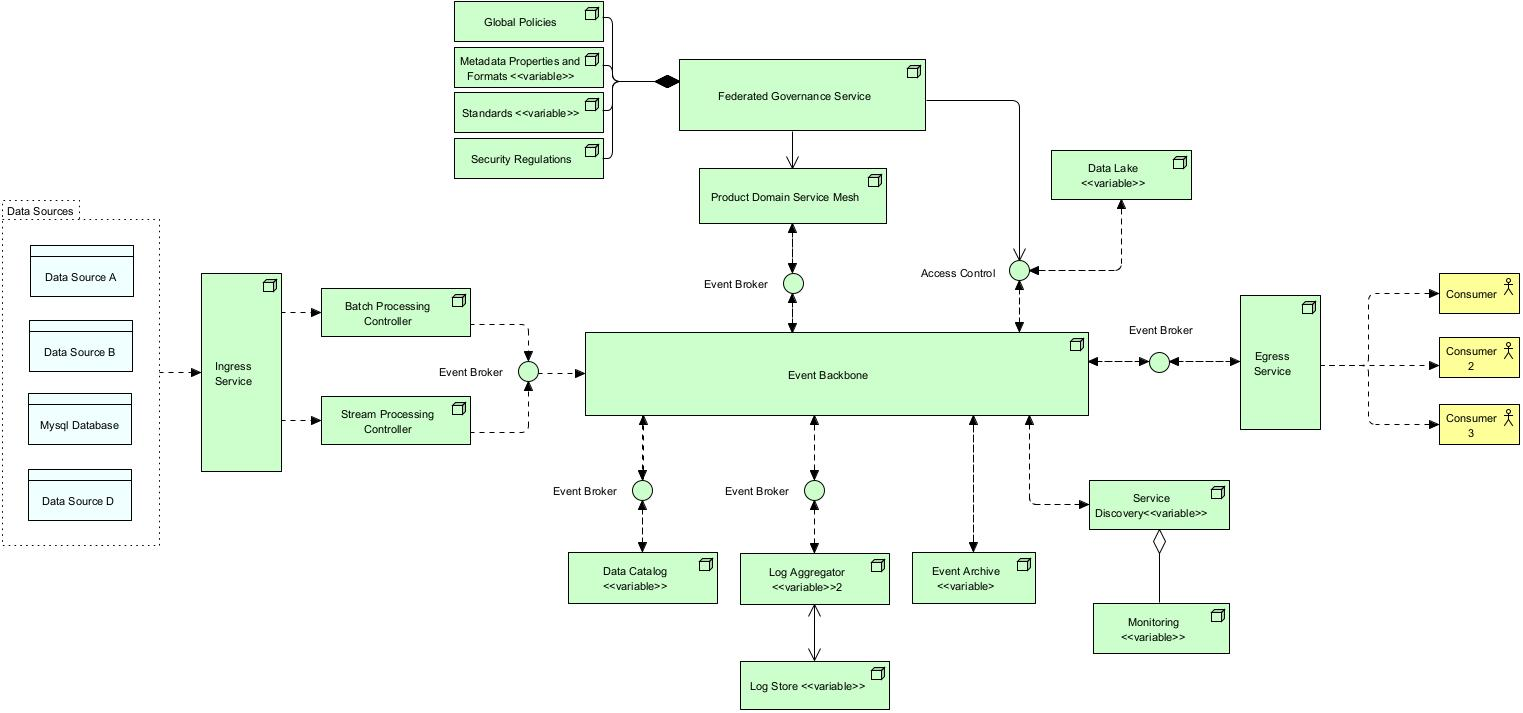
\includegraphics[width=12cm]{media/Metamycelium.jpg}
    \label{RA}
    \caption{Domain Driven Distributed RA}
\end{figure}



\begin{enumerate}
    \item \textbf{Ingress Service:} this service is responsible for controlling traffic into the system. Depending on the nature of the request, this service will load balance either into a batch processing controller or a stream processing controller. Ingress is an asynchronous load balancer designed to eliminate choke points, handle SSL termination, and provide with extra features such as named-based virtual hosting. 
    
    % Having defined ingress allows for clear demarcation of the system boundaries, eliminates performance affecting security measures to be taken care of, allows for more private networks within the system, and can be used to augments objects too. 

    \item \textbf{Batch Processing Controller:} this controller is responsible for handling batch processes. That is, it is responsible for receiving request for batch processing, and communicating it to the event broker. Due to the batch nature of the requests, the controller can decide to achieve this in a bulk and asynchronous manner. 
    
    % This controller as opposed to its stream processing counterpart, can execute non compute-intensive proxy operations if needs be.
    \item \textbf{Stream Processing Controller:} This controller achieves similar thing to the batch one, with a difference that it has to handle a different nature of requests. Stream events are synchronous in nature and require hight through-put. Having a specific service for stream processing requirements promote tailored customization that best suit the varying nature of stream events. 
    \item \textbf{Event Broker:} event broker is an important architectural construct designed to achieve 'inversion of control'. As the system grows, more nodes and services are added, communication channels increases, and there is a need fore new events to be dispatched. As each service communicates through the event backbone, each service will be required to implement it's own event handling module. This can easily turn into a spaghetti of incompatible implementations by different teams, and can even result in unexpected behaviors. To address this issue, an event broker is introduced to each service which has one main responsibility; communication with event backbone. 
    
    % This means services are no longer required to implement their own event handling functions, and this responsibility is given to the event broker instead. One of the key success criteria for event brokers is a unified interface that resides in a right level of abstraction to account for all services of the architecture.
    \item \textbf{Event Backbone:} Event backbone is the heartbeat of the system, facilitating communication between all services. Where as this service is displayed as one technology service in the Archimate diagram, we recommend the event backbone to be designed underlying distributed paradigms itself. This is to ensure scalability as the number of topics and events grows. Event backbone and its relations to other nodes is analogous to a dance troupe; in a dance troupe, the members respond to the rhythm of music by moving according to their specific roles; the same happens here, with a difference that this time, event backbone is the music and services are the members of the dance troupe. This implies that services are only responsible for dispatching events in a 'dispatch and forget' model, subscribing to topics they are interested. 
    
    % Whereas networking challenges remain the same, this approach solves myriad of challenges associated with point-to-point communication.
    \item \textbf{Egress Service:} This services is responsible for providing necessary APIs to the consumers of the system, third parties or other big data systems. This allows for the openness of the architecture, and lets data scientist and business analyst easily request the data necessary for their work-loads. This also promotes the idea of self-serve-data through service discovery, data catalogue and product domains. This component can also be tuned for QoS networking, and other low computational functions if needs be.
    
    % Systems or scientists can first request for a data catalogue and then use the catalogue to request for the required data. The egress services handles the traffic necessary for these requests to be successful. This component can also be tuned for QoS networking, and other low computational functions if needs be. 
    \item \textbf{Product Domain Service Mesh:} Driven by the idea of domain-driven design, every product has it's own bounded context and ubiquitous language, and is technically governed by a service mesh. Every service mesh is made up of a batch ingress, stream ingress, big data storage, big data processing framework, domain's data service, together with the control tower and the side cars. These components provides the necessary means for the domain to achieve its ends in regards to big data processing. This is to enable high cohesiveness, low coupling and clear interfaces among services. 
    \item \textbf{Federated Governance Service:} Given the distributed nature of the architecture and sheer number of moving parts with varying life-cycles; there is a need for some global contextual standards and policies that are designed to streamline processes and avoid losses. This is not to limit the autonomy of teams, but to inject them with best practices and organizational policies that tend to reflect the capability framework, regional limitations, and legal matters that can cause sever damage to the business. 
    
    % For instance, not every data engineer may be fully aware of various aspects of GDPR, or different teams may choose to embark on different event deduplication processes; for the former, one can adopt a global privacy policy rule, and for the latter, one can pick up Async API specifications. 
    \item \textbf{Data catalog:} As data products increase in the system, more data become available, interoperability increases, and thus services have to know who provides what data. Data catalog is responsible for keeping a catalog of all data available among services with relative paths to fetch those data. 
    \item \textbf{Log Aggregator and Log Store:} Operating underlying a distributed paradigms, requires a shift in a way that logging occurs. This means system cannot rely only one applications reporting logs in a single environment, but there's a need for a distributed tracing that shows a lifecycle of a process and how it went through different services. Therefore this RA benefits from the popular log aggregator pattern initially released by the microservices community, to allow fo graceful scaling of system's logging strategy. 
    \item \textbf{Event Archive:} One of the main challenges of this architecture is it's reliance on event backbone. Whereas event backbone itself is recommended to be distributed and fault tolerant, event archive further solidifies the service recovery from unexpected events. This implies that, if the event backbone went out of service, the history of events can be stored and retrieved from the event archive to bring various services to the current state of operation. 
    \item \textbf{Data Lake:} Whereas product domains are demarcated and boundaries are well-defined, we do not find it necessary for each domain to maintain it's own data lake. This is under the assumption that a lot of data is now processed at the time of storage, and is required whenever there is a analytical business case for it. Whereas there isn't a data lake per domain, different domains can have a quota in the data lake that is owned and handled by access control. 
    \item \textbf{Service Discovery:} In a distributed setup like the one portrayed, services need to find each other in order to communicate their means. 
    
    % A naive way to achieve this could be the storage of service addresses in configuration files in services interested to know about a particular service. This soon becomes out of hand, is hard to scale and hard to maintain. 
    
     Service discovery solves this issue with primary responsibility of identifying services and answering queries about services. This is achieved by services registering themselves to service discovery on boot up.
    \item \textbf{Monitoring:} Last, but not least, in order to take proactive measures for the overall health of the system and its considerable moving parts, one needs to actively monitor the state of the individual nodes and the overall flow of things. Services emit large amounts of multi dimensional telemetry data that can be read and analyzed for the supporting actions. Monitoring services help storing these data to fuel proactive actions. 
\end{enumerate}

The elements of the RA that are annotated with the phrase 'variable' can be modified, adjusted or even omitted based on the architect's decision. It is als worth mentioning that what's provided is a brief explanation of these elements, and each element's description can be extended to a considerable amount. 

% The aim of this RA is not limit the creative of software architects, but to facilitate their decision making process. 

 

\section*{Evaluation:}

Of utmost importance to development of the RA, is the evaluation of it. Our aim is to evaluate the correctness and utility of the RA by how it can turn into a context-specific concrete architecture that solves an actual problem. ATAM can increase confidence in the RA, by appraising architectural decisions and their consequences on the system. 

% For brevity purposes, we dot not expand on ATAM steps in detail or the benefits of it, and we only explain how the evaluation has been conducted. Some details of this evaluation is omitted to protect the security, and intellectual property of the practice, and some details are modified for academic purposes. These modifications have not affected the integrity of the evaluation.  

\subsection{Phase 1:}
Evaluation has taken place in a subsidiary of an international large-scale company. The subsidiary company is specialized in practice management software for veterinary professionals visa Software as a Service ( SaaS ) providing services to hospitals all around the globe, among which is some of the biggest equine hospitals, and universities. The company has several ambitions, one of which is big data an AI. 

Following the guidelines of ATAM, the first step was the identification of relevant stakeholders. Our emphasis was on key stakeholders such as lead architects. This was important to ensure that we have not missed anything major in our design. We also opted not to include stakeholders that do not directly correlate with the RA, such as the UI/UX designer. As a result we invited two lead development architects, head of product, a product owner responsible for the product in which the artifact is tested, a quality assurance engineer and several developers. 

During the initial meeting, ATAM was presented with clear description of its purposes. From there on, the RA has been discussed, our assumptions have been stated, and variability points portrayed. In the second half, stakeholders discussed the background of the business and some of the challenges faced, and the current state of affairs. After that, the stakeholders unanimously selected a few business case that are the most relevant to the purposes of this study. 

\subsection{Phase 2:}

After the selection of appropriate scenarios and several good cases for BD processing, we instantiated a prototype of the RA. We utilized ISO/IEC 25000 SQuaRE standard (Software Product Quality Requirements
and Evaluation) \cite{ISO25000} for technology selection. This prototype is a partial instantiation of the RA, that is aimed to solve a context specific problem. 

% We found mature technologies that could support our requirements, and opted not to develop any tools from scratch for the purposes of this study. It is also worth mentioning that, 

As for the technology choices, we chose Node JS for all APIs and custom scripting, Nginx as our ingress, AWS Lambdas for stream and batch processing controllers, Kafka for event backbone, Kafka event brokers as the event broker, AWS application load balancer as the egress load balancer, Istio as the control tower, Envoy as the side car, Kubernetes as the container orchestrator, AWS S3 as the BD store and event archive(we used company's already in production data lake, with a test bucket in a staging environment), and Data Bricks for stream and batch processing. 

We aimed to incorporate most components of our RA into this instance, however logging, monitoring, service discovery, federated governance service, and data catalog has been omitted. After this step, we presented the prototype, discussed our technology choices, highlighted quality attributes, and clarified confusions, questions. 

\subsubsection{Identifying Architectural Approaches:}

In this step, we discussed architectural styled in regards to quality attributes. We classified our architecture as micro-services. This was easier to grasp than 'domain-driven distributed architecture' for the stakeholders. For availability, we discussed Kafka's partitions, Nginx worker connections, Data Lake and Istio.  For performance, we discussed Nginx asynchronous processing, Kafka topics and consumers, AWS application load balancer, and Kubernetes pods. For modifiability, we discussed the concept of domain driven design, side cars, and event brokers. 

We then continued to analyze these approaches for tradeoffs, sensitivity points, and potential risks. 

\subsubsection{Scenario Prioritisation: }

Scenarios are the quanta of ATAM, and help capturing stimuli to which the architecture has to respond. Based on this premise, in this step, we asked stakeholders to priorities three class of scenarios namely 1) growth scenarios, 2) use-case scenarios and 3) exploratory scenarios. As a result of this we pooled 20 requests, which we then asked stakeholders to vote on. The voting process yielded 5 scenarios, described as two user journeys; 1) The pet owner brings the pet to the veterinary hospital, the pet is diagnosed with cancer. The pet's environmental factors should be studied for potential clues on the root cause of cancer; 2) A pet owner brings the pet to the veterinary hospital, the cat symptoms should be processed for early detection of lyme disease. 

\subsubsection{Utility Tree Elicitation: }

In order to generate the utility tree, we first needed consensus on the most important quality attributes for this evaluation. We presented our assumptions and after a discussion, despite the fact that there was some concerns over privacy, the members agreed on availability, performance, and maintainability as the most important quality attributes. Based on that, we created the utility tree with the requirements of; 1) performance: system should be able to process real time streams under 1200 ms, 2) availability: load balancer and data bricks cluster being available 99.999\% of the time, and 3) modifiability: new service mesh to be added with less than 2 person a week.

\subsubsection{Analyze Architectural Approaches: }

After identifying architectural approaches and prioritizing scenarios, we ran the scenarios against our prototype. This is to provide heuristic qualitative analysis and point out sensitivity points and tradeoffs. We initiated this process by creating a custom script that extracts actual data from the company's mySQL database, and send it through the ingress. We create the necessary topics for Kafka, and configured Nginx to pass the requests to responsible lambdas for batch and stream processing. We then followed with event producers, Istio, Envoy, Kubernets, Data Bricks and the rest of the system. 

In the process of running the scenario simulations against our system, we constantly probed our architectural approaches. Many implementation details arose in the process, and many sensitivity points annotated. We realized the true cost of the system, its trade offs and potential challenges. Based on these premises, and stakeholder feedbacks, we deduced that system quality Q\textsubscript{S}, is a function f of the quality attributes performance Q\textsubscript{P}, availability Q\textsubscript{A}, and modifiability Q\textsubscript{M}, as the equation Q\textsubscript{S} = fQ(Q\textsubscript{P}, Q\textsubscript{A}, Q\textsubscript{M}).

For performance, we used the cloud stress testing agent called StressStimulus. We ran the stress test against our system a couple of times, which revealed some interesting insights. It became evident that cold start time (100-1000ms) of AWS Lambdas can affect the desired performance. On the other hand, using Data Bricks for stream processing, we opted not to use micro-batch to have an accurate evaluation, we also decided not to configure the fair scheduling pool, so as to test the worst case scenario. 

% One solution to this was replacement of Lambdas with EC2 instance, but we opted not to do that, because this would affect maintainability negatively, as each EC2 instance needs provisioning and maintenance. 

After analyzing the prototype with various performance models (periodic data dispatch, large volume of data, many concurrent requests), it became evident to us that latency, input/output, and object mutations were the performance sensitivity points. The event driven nature of the system really shined at handling various simulations. Based on these findings, we characterize system's performance as  Q\textsubscript{P} = h(l, s, c). That is, system is sensitive to latency (l), side effects (s), and concurrency (c).

Next, we tested our prototype from availability point of view. Since the system is distributed in nature, the failure in one service, if not handled properly, can have a ripple effect on all services. Our prototype could easily recover from such situation through implementation of circuit breakers in event brokers. Our prototype also archived the events before the failure occurred in the event backbone, to bring back the system to a correct state. Moreover, we set up health checks and alarms on pods in the Kubernetes cluster and constantly monitored for system behaviors. 

% Another area were we initially worried a lot about, was the event backbone and fear of it turning into ESB of SOA, but that was certainly not the case, given that we designed the RA with the idea of a distributed backbone in it self. 


Kubernetes made sure that certain amount of services are always available through special services called deployments and replica sets. This evaluation has also made us realize that our architecture is compliant with twelve factor methodology and can be deemed cloud native. This has positively affected the availability score. Given all, we characterize the system's availability as $Q\textsubscript{A} = g(\mu\textsubscript{C}, \lambda\textsubscript{E}, \mu\textsubscript{S})$. That is, system availability is affected by the time it takes for circuit breakers to trip and become available again ($\mu\textsubscript{C}$), failure of the event backbone ($\lambda\textsubscript{E}$), and the it takes for the services to recover ($\mu\textsubscript{S}$), with g being fraction of time that system is operating.

Lastly, we tested our prototype from modifiability point of view. The distributed and domain driven nature of our architecture allowed us to easily achieve the desired modifiability objectives and even beyond. Adding a new service mesh only required us to extend our HCL module written in Terraform for our EKS cluster, and modify it with new Docker images. Brokers were also streamlined, so we could spin up a new broker within minutes. We did not have to worry about certification lifecycle as it was handled by Istio, Local Cert Manager and Let's Encrypt. 

% Areas that we found more challenging was a bit more vendor specific. For instance, Databricks cluster optimisation, configuring Nginx as EKS ALB ingress, and handling ECR secrets and having them stored as Kubernetes secrets was not straight forward. 

Taking all into consideration, we characterize system's modifiability as $ Q\textsubscript{M} = s(K, K, D)$. That is, system modifiability is sensitive to Kafka provisioning, maintenance and configuration, Kubernetes maintenance, provisioning and configuration, and Databricks provisioning, configuration and maintenance, with s being the skill set required. 

\subsubsection{Tradeoff Points:}

After clear analysis, two tradeoff points have been identified; 1) event brokers and the event backbone and 2) service mesh. One area that raised concerns was the event backbone, and how it might turn into a bloated architectural component analogous to ESBs in SOAs. However, given the distributed nature of the system, event archive, and event brokers, we do not find that likely to happen. This architectural component is designed itself underlying the distributed principles and is responsible only for one function; communication among services. In addition, in the case of service outage, event archive can be utilized to retrieve the order of events, which in turn brings system to a correct state. Event brokers on the other hand, facilitate modifiability by providing native event handling mechanisms, but at a cost of one more layer and potential latency that comes with it. Given these, we deduced that event backbone while affecting performance and maintainability positively, can potentially have negative impact on availability and reliability. 
 
% During the tradeoff discussions, many other quality attributes have been discussed that are omitted for the purposes of this study. 
On the other hand, we realized, event brokers have positive effect on modifiability and availability, without having much negative effect on performance. One other area that was discussed heavily was the service mesh. Many developers found a lot ot be done before the service mesh can operate and be up and running. We argued that while the initial effort for bringing up a service mesh may sound daunting, modifiability is positively affected longitudinally. Service mesh also promoted the concept of clear interface, separation of concerns, and a well-defined bounded context. 

% It also freed many developers from platform work that they usually don't excel at. 

Based on that, we deduced that service mesh has affected modifiability positively, but it might affect performance and reliability negatively due to the communication required among services. 

%  Given all, even though we designed our RA with event back bone or a service mesh, we do not strongly prescribe these pattern. Our aim is not kill to creativity of software architects, but to shed lights on new ways of doing things with battle proven patterns. 
 
 Two limitations discussed among stakeholders was 1) complexity of implementing the design and 2) tail latency. For the former, we do not think that a distributed big data architecture should be simple; we simply do not recommend organizations to embark on this journey if they do not have the resources necessary to absorb the complexity. For the latter, we do not have a straight forward solution. This is a well known issue in the microservices community as well, and is addressed in our design by the means of fault-tolerant services.  
 
%  Howbeit, if the company can absorb the complexity, they will gain significant competitive advantage. 
 


 \section{Conclusion}
  
 Big data engineering is sophisticated process, and while there are many good practices institutionalized in software engineering, data engineering domain does not seem to benefit from all of it. This has led to several challenges in development of BD systems, and many companies have failed to bring to light the potential of a data-driven decision making. We aimed at facilitating this process in this study by proposing a BD RA. Nevertheless, there's more and more research required in the area of data processing, reactive event driven data processing system, data engineering and big data architectures. Some areas that need considerable attention is security, privacy, and metadata management for big data architectures.

%
% ---- Bibliography ----
%

\bibliographystyle{splncs04}
\bibliography{mybibfile}
\end{document}
